This chapter will describe the design and implementation of the application which is composed of a representational state transfer (REST) application program interface (API) and a front-end (FE) web application. 

\section{API}
Since the scraped pages of the dark-web were stored via ElasticSearch it was necessary to create a back-end application (BE) in order to perform various operations on the data-set before sending it to the FE. We decided to create a Python BE since the application had to be able to run on a UNIX system. 
\subsection{Technology overview}
Python is a widely used interpreted programming language known for its  readability and portability \cite{aboutPython}. It is open-source and is considered to have an extensive documentation and community available. Another huge advantage is its popularity in the science community. Because of this there is a great amount of useful libraries for research purposes such as NetworkX\footnote{A library used for creating and working with graphs.} \cite{networkX} or cylouvain \footnote{A library with a fast implementation of LA.} \cite{cylouvain}.  
As we wanted to follow the REST architecture we decided to make use of the Django framework \cite{meetDjango}. It is responsible for tasks such as running the server or managing web requests. Another advantage of Django is its Django REST framework (DRF). DRF offers a convenient way for creating restful endpoints and responses. \cite{djangoRest}. Both frameworks are open-source again with extremely helpful documentation and community. 


Because it takes approximately 60 seconds to retrieve about 90,000 pages from the database and circa 13 seconds to divide such a response into communities, caching had to be introduced. For that purpose Redis \cite{redis} is used. It is an open-source solution which we use as a key-value store. It supports  basic data structures as values, e.g. strings, numbers or sets but not custom objects. Since the API uses custom objects for both communities and pages, an object serializer had to be leveraged along with Redis. We decided not to write our own but to utilise the python pickle module \footnote{A module used for converting python objects to streams of bytes and vice versa.} \cite{pickle}. 

\section{Front-end}
For users to be able to see the data acquired from the BE in a reasonable way a FE application was created. 
\subsection{Technology overview}
The probably most favoured programming language used for creating web applications \cite{jsGithut} is called JavaScript (JS) \cite{javaScript}. It is an interpreted language supported by all modern browsers. It is open-source and as such disposes of a big community with splendid documentation. Because it is not strongly typed the code might be complicated to read or navigate. For this reason the FE was written in TypeScript (TS) \cite{typeScript} which is a superset of JS with the advantage of being typed. Both JS and TS come with a significant amount of tools used for implementing user interfaces (UI) in a clean and timely manner. One of the most favoured frameworks is React.js \cite{react} which when used correctly results in readable code and improves performance by managing the re-rendering of page elements.


To be able to supply the FE with the needed data for user interactions a store had to be implemented. React.js and TS work extremely well with a state container called Redux \cite{redux} and because of that we decided to leverage it. It is centralized with only one store, easy to debug and again has a convenient documentation. 

The doubtlessly most important part of this FE is the visualization of the graph built on the data sent from the BE. This feature is built using the react-d3-graph library \cite{reactD3Graph} which is 
an implementation of the library d3.js \cite{d3} made more convenient for the use with React.js. 

\subsection{User interface}
After the application is loaded the UI is composed of a header with the name of the application "Dark web categorization" a loader and a sidebar in the right hand side with several inputs or buttons in a column as can be viewed in figure \ref{zeroLevelGraphBasic}. At the very top a drop-down button is present which enables the user to filter the data. Underneath it an input field for filling in a search phrase with a submit button next to it for filtering out a single node or multiple nodes with which the search phrase matches is situated. The last element shown is an indicator of the current level the user is observing which at the beginning is zero. 
\begin{figure}[ht!]
  \centering
  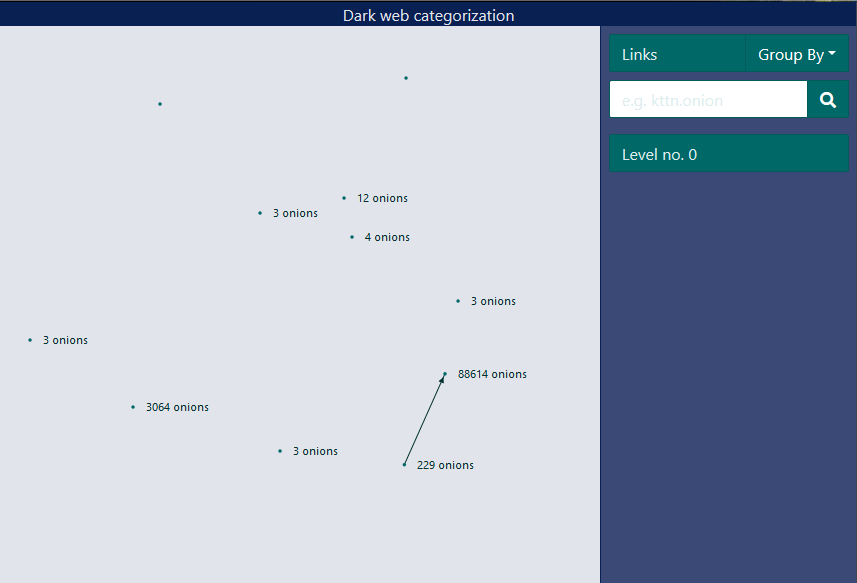
\includegraphics[width=\textwidth]{Images/ZeroLevelGraphBasic.png}
  \caption{The basic view of the app with a selected community and its details.}
  \label{zeroLevelGraphBasic}
\end{figure} 


The moment the data is retrieved from the BE the loader gets replaced for a graph which represents the communities the pages are partitioned into or the pages themselves and the links between them. Each node is displayed as a pie chart of categories of the pages belonging to the community represented by the node (CRN) or the page itself. There also might be a mock-community visible containing isolated nodes which cannot be zoomed into. It is possible for a level to depict communities and pages at once. 


After single-clicking a node additional information is exampled in the sidebar.The details vary depending on whether the node is representing a community or a single page.  
The details of an individual page are as follows: 
\begin {description}
	\item [Url] which also serves as a unique identificator of the page. 
	\item [Category] of the page. Each page belongs to one category.
	\item[Links] to other pages displayed as a list of url addresses. There are up to ten links visible in the sidebar. The remaining links, if any, are downloadable in a text file. 
	\item[Content] of the page if it is available. If the content is too long to be disclosed in the sidebar it is again downloadable in a text file.
\end{description}


The details of a community consist of  grouped information of its pages and include the following:
\begin {description}
	\item [Category composition] which is aggregated from the categories of all the pages of the community. Each category is represented by its name and the percentage of its relevance in the community.
	\item [Page urls] belonging into the community. There are up to ten urls visible in the sidebar. The remaining pages, if any, are downloadable in a text file. 
	\item[Urls count]represents the number of all the pages belonging into the community. 
\end{description}


The CRN needs to be double-clicked in order to zoom into a it to view its sub-communities. If the current level is higher than zero a button for zooming out appears next to the level indicator. It is shown in figure \ref{levelIndicatorWithButton}.
\begin{figure}[ht!]
  \centering
  
\includegraphics{Images/levelIndicatorWithButton.png}
  \caption{The level indicator with the zoom-out button. After the zoom-out button is clicked, the user is shown the communities of the previous level.}
  \label{levelIndicatorWithButton}
\end{figure} 


The user is able to zoom into the very last level (maximum level) where only individual pages are displayed. Each community may have a different maximum level, depending on its pages and structure.


